The following is a representation of the tasks with Gantt graphs, its expected that the work is done on weekdays at 8 h of work a day. The figures don't account for possible holidays for software limitations. In addition the project is expected to be finished before schedule. This is to accommodate probable delays in software development or the experiments. Figures \ref{fig:GanttRLCI}, \ref{fig:GanttSIP} and \ref{fig:GanttTAC} show the schedule defines according to Section \ref{sec:Tasks}

\begin{figure}[h]
        \centering
        \centerline{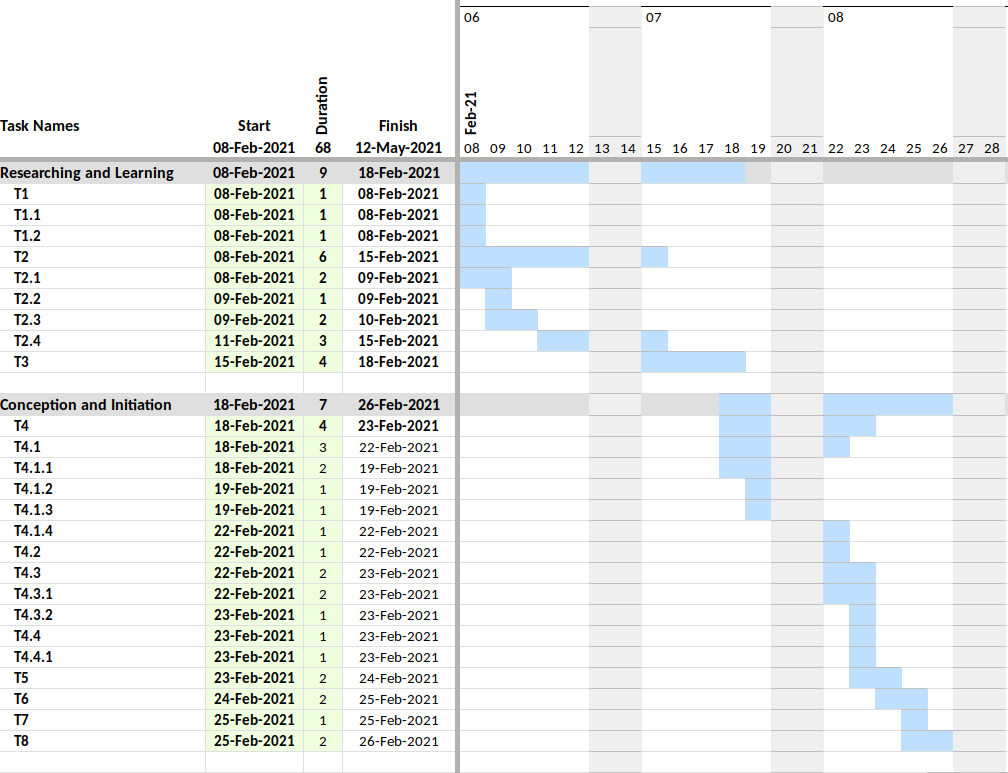
\includegraphics[scale=0.45]{Figures/Gantt_RL_and_CI.png}}
        \caption{Gantt of the first two sections: \textit{Research and Learning} and \textit{Conception and Initiation}}
        \label{fig:GanttRLCI}
\end{figure}

\begin{landscape}

\begin{figure}[ht]
        \centering
        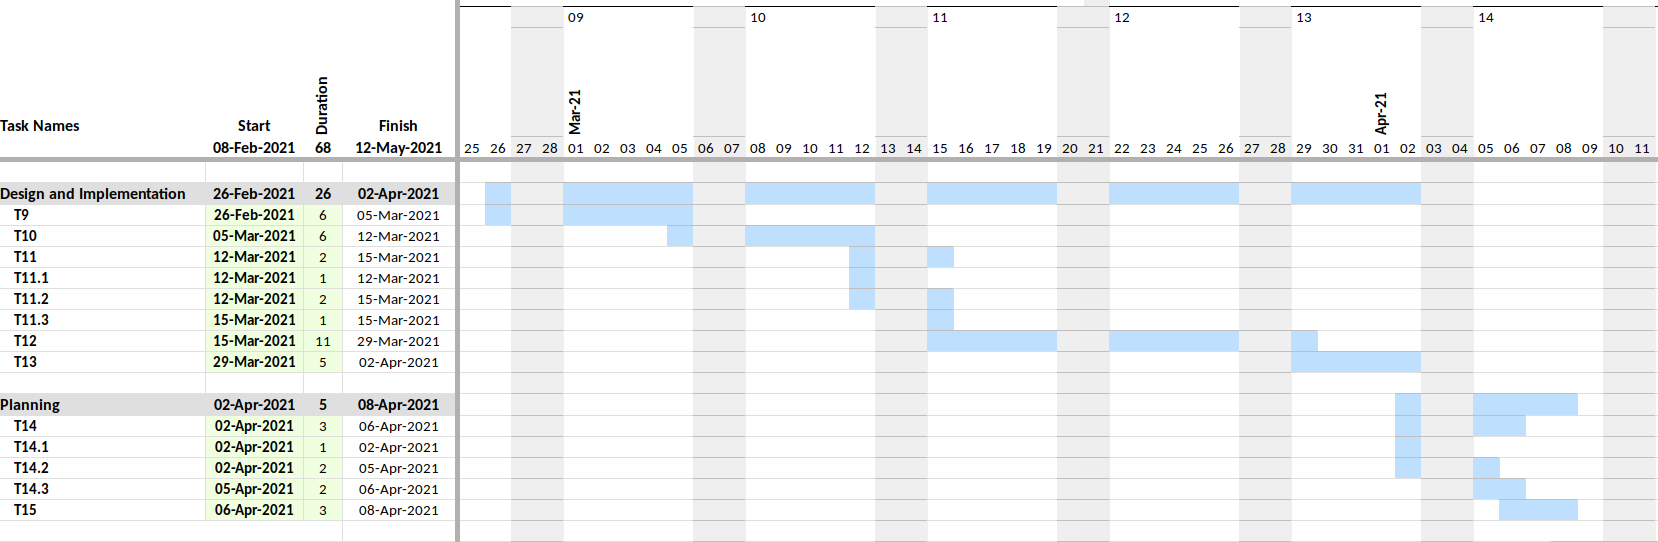
\includegraphics[scale=0.27]{Figures/Gantt_SI_and_P.png}
        \caption{Gantt of the middle two sections: \textit{Design and Implementation} and \textit{Planning}}
        \label{fig:GanttSIP}
\end{figure}

\begin{figure}[ht]
        \centering
        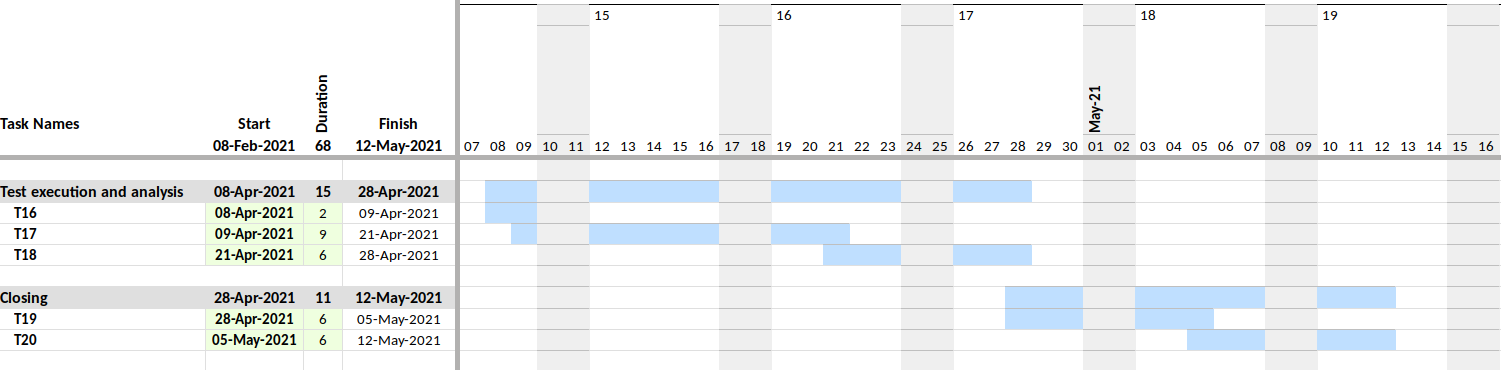
\includegraphics[scale=0.29]{Figures/Gantt_TA_and_C.png}
        \caption{Gantt of the middle two sections: \textit{Test execution and analysis} and \textit{Closing}}
        \label{fig:GanttTAC}
\end{figure}

\end{landscape}